\setcounter{chapter}{4}

\chapter{Coopetitive Behavior of Services within Communities}\label{cha:PCTLKC}


\section{Introduction}

In the previous chapter, our focus was on community formation and we emphasized cooperative behavior of the web services as agents. Within communities, the web services, selfish and utility maximizers by nature, can follow two different strategies, namely cooperation and competition in order to increase their payoffs when they provide services to consumers \cite{VuFind-10008938119}. In typical business settings, services are used to compete within communities as they provide the same functionalities and the number of users requests is finite. However, the same reason of providing similar functionalities can lead services to cooperate because they can replace each other in case of failure or unavailability, and services can do better in a coalition structure. Analyzing services competition and cooperation strategies within communities is still an open problem that motivates the research described in this section. we propose a mechanism within which service agents
in the community could choose either to compete for an announced task\footnote{Requests and tasks are used in this report interchangeably.}, or to cooperate with other competing services in the same community to accomplish some subtasks of the announced task. We equip intelligent web services to follow a reasoning technique to choose best interactive strategy (Coopetitive attitude, which is categorized to compete and cooperate). In the proposed system, We explore details behind the strategic decision making procedures and enable service agents to apply different techniques to constrain high efficiency and obtain the maximum utility. We investigate services' expected payoffs and the involved probabilities that are used to choose over the two interacting strategies.



%\subsection{The Proposed Framework}\label{The Proposed Framework}
Here, we first present the architecture of the proposed
model. We explore the characteristics of intelligent service
agents and their network. We link this architecture to the
implemented system where we investigate the services' coopetitive
attitudes. We compute the involved system parameters and explain
the services' interactive strategy profiles by highlighting their
coopetitive choices.



\begin{figure}[h]
\centering
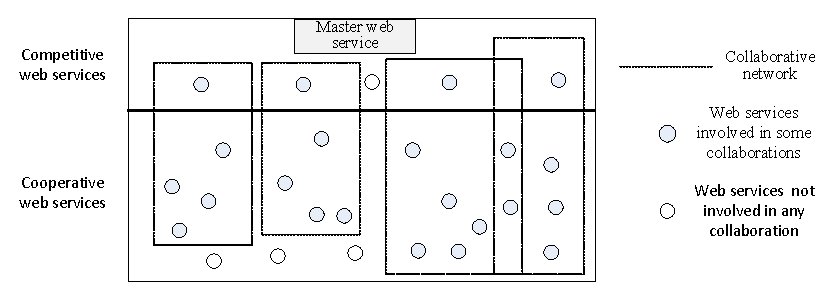
\includegraphics[scale=1]{Figures/architecture++.eps}
\caption{Services are partitioned into competitive and cooperative
sets. Competitive services may get tasks directly from the master
agent and they can share it with other cooperative services in
their collaborative networks within the same community.}
\label{architectureFigure}
\end{figure}

\section{Architecture}

Figure \ref{architectureFigure} illustrates the architecture of a
typical community aggregating a number of services with different
interactive strategies. Some of them compete for the task where
they directly deal with the master. Some others cooperate in the
associated task where they only deal with the competed service as
the task leader and do not directly interact with the master (the
master deals only with the service that has bid for the task,
which is responsible of choosing its collaborative network). In
both sets, some service agents are for certain moments out of any
collaboration network. Upon allocation of
the task, the service is responsible for offering the required QoS
that is stated in the task being generated by a consumer.
Afterwards,  the master rewards or penalizes the competing
service by upgrading or degrading its reputation according to the
offered QoS compared with the required one. This comparison
influences the sorting mechanism used by the master to allocate
the tasks in further task allocation rounds.


%ok til here


\section{System Parameters}
In this section, we demonstrate the involved parameters and their
corresponding formulations and explanations.

\textbf{Task QoS} ($T_{QoS}^r$) is the required QoS metric for a
specific task $r$. Users define tasks with specific QoS
requirements such as response time, availability, and
successability (or accuracy). We aggregate and
normalize these metrics to a value between $0$
and $1$. %Throughout this paper, we refer to this value as
%$T_{QoS}$.

\textbf{Service QoS} ($QoS_w^r$) is the QoS provided by the
service $w$ after performing the task $r$. Again, the metrics that
contribute in computing this QoS are aggregated and normalized to
a value between $0$ and $1$. The offered quality might or might
not meet the required task quality $T_{QoS}^r$. In the latter
case, the service user would be disappointed and a negative
satisfaction feedback is expected. In our proposed system, both
cases are considered when calculating the services' reputation.

%\textbf{NTD} is the number of tasks completed by a web service.

\textbf{Budget} ($B_w^t$) is the amount of money the service agent
$w$ has in its disposal during the window time $t$ (i.e.,
$[0,t]$), which helps pay for the community membership fees
($\epsilon$) and is one of the parameters that the service agent
considers when deciding about getting involved in a competition or
not.

\textbf{Reputation} ($Rep_w^t$) is a significant factor in any
online community \cite{Fouss:2010:PRM:1751668.1751727}. Without a reputation enabling
mechanism, users cannot differentiate among services, specially
the ones which offer the same type of service. Reputation
mechanisms usually aggregate users' experiences and in our case it
strongly depends on QoS that each service provides. Users define
tasks, each one with specific quality $T_{QoS}^r$, so that after
performing a certain number of tasks, each one with $QoS_w^r$,
during a window time $t$, the reputation of $w$ gets evaluated by
the master agent. $Rep_{w}^{t}$ refers to the reputation of $w$
during that window time $t$.

In Equation \ref{repr}, we compute the reward that the master
computes considering the task $r$'s QoS $T_{QoS}^r$ compared with
the service offered quality $QoS_w^r$. In case the offered quality
meets user expectations, the reward value would be positive. In
this system, we consider a small value as default rewards $\eta$
which the master considers together with the proportional level of
satisfaction as a weighted value (by $\upsilon$). In this case,
the higher the offered quality, the more weighted reward. In case
the offered quality did not meet the user expectations, the reward
would be negative. A default penalty value $\rho$ (where
$\rho>\eta$) together with the weighted proportional difference
are therefore considered. The idea is to harshly penalize the
services rather than rewarding them. To this end, rational service
agents should carefully analyze their capabilities once the
available tasks are announced. Equation \ref{reward} computes the
obtained reward by $w$ during the window time $t$ considering the
set $task_w^t$ of tasks performed by $w$ during the window time
$t$. In our proposal, service agents have the goal of increasing
their budget, which is directly related to their reputation. Thus,
they have to decide strategically how to maximize this value.

\begin{equation} \label{repr}
reward_w^r = \begin{cases}
\eta + \upsilon \frac{QoS_w^r}{T_{QoS}^r+QoS_w^r}   & \text{if $T_{QoS}^r\leq QoS_w^r$;}\\
-(\rho +  \upsilon \frac{T_{QoS}^r}{T_{QoS}^r+QoS_w^r} ) & \text{otherwise.}\\
\end{cases}
\end{equation}


\begin{equation} \label{reward}
reward_w^t =
\begin{cases}
\frac{\sum_{r \in
task_w^t}reward_w^r}{|task_w^t|}& \text{if $task_w^t \neq \emptyset$;}\\
0 & \text{otherwise.}\\
\end{cases}
\end{equation}

The assigned reputation value is updated by the computed reward
value. The computed reputation of services is bounded by the
minimum and maximum reputation values $0$ and $1$. % to constrain
%the balance the cooperative community of web services. The updated
Let $\Gamma = Rep_{w}^{t} + reward_w^t$. The updated reputation
value is then computed as follows:

\begin{equation}\label{repz}
%Rep_{w}^{t+1} = Rep_{w}^{t} + reward
%\end{equation}
%\begin{equation*}
Rep_{w}^{t+1} = \begin{cases}

\Gamma & \text{if $ 0 \leq \Gamma \leq 1$;}\\
0  & \text{if $\Gamma < 0$;}\\
1 & \text{if $\Gamma > 1$.}\\
\end{cases}
\end{equation}
%
For new services with no previous reputation value, we use the
bootstrapping trust technique proposed in \cite{DBLP:conf/icwe/YahyaouiZ11}. This
technique consists in giving the new services a chance and observe
their behaviors for a period of testing time. The observation
sequence is modeled as a hidden Markov model that is used to
detect the behavior of the service by comparing the observation
behavior against pre-defined trust patterns. Based on the matching
result, an initial value is assigned to the service. Using this
initial reputation value, services quickly converge to their
actual and stable values using the update function.

\begin{proposition}\label{Complexity-Rep}
$Rep_{w}^{t}$ can be computed in time $O(|t|)$, i.e., in time
linear in the size of the window $t$.
\end{proposition}

\begin{proof}\footnote{In this work, we
assume that the common arithmetic and elementary functions, such
as multiplication, division and trigonometric functions can be
computed in time $O(1)$ as they operate on inputs of fixed sizes.}
The function $Rep_{w}^{t}$ is recursive on $t$, but the algorithm
works by storing the last calculated reputation value in a
variable, so it will not be recalculated again at each iteration.
However, the calculation of $reward_w^t$ is needed. Since the
function $reward_w^t$ can be computed in time linear in the number
of tasks (see Equations \ref{repr} and \ref{reward}), which in
turn is linear in the size of the window time, the result follows.
$\Box$
\end{proof}

\textbf{Growth Factor} ($G_w^t$) is a parameter which declares
services' performance based on their recent strategies and
activities. Growth factor is relative to services' reputation
$Rep_w^t$, QoS during the window time $t$ $QoS_w^t$, and budget
$B_w^t$. This factor is the main variable a typical service uses
to decide about which strategy to adopt. We use Equation \ref{eq:growthfactor} to compute the
growth factor $G^t_w$ of the service $w$ during the window time
$t$ as the average of the three aforementioned parameters, where
$n_t$ is the total number of offered tasks to the whole community
during the
window time $t$, %(we consider the time window $t$ large enough so
%that $n_t \neq 0$),
$\mu_w$ is the mean received service fee, and $\epsilon$ is the
cost of community membership.

\begin{equation}\label{eq:growthfactor}
G^t_w = \frac{Rep^t_w + QoS_w^t+\frac{B_w^t}{n_t  \mu_w -
\epsilon}}{3}
\end{equation}
\begin{equation*}
\mu_{w} \in\{\mu_{w, CM}, \mu_{w, CO}\},~~~QoS_w^t =
\begin{cases} \frac{\sum_{r \in
task_w^t}QoS_w^r}{|task_w^t|}& \text{if $task_w^t \neq \emptyset$;}\\
0 & \text{otherwise.}\\
\end{cases}
\end{equation*}


This equation is designed so that it satisfies the following
desirable properties:

\begin{enumerate}

\item The growth factor function should be monotonically
increasing in the offered quality of service $QoS_w^t$.

\item The growth factor function should be monotonically
increasing in the service's reputation $Rep^t_w$.

\item The growth factor function should be monotonically
increasing in the budget $B_w^t$ if the maximum possible profit is
positive and monotonically decreasing in $B_w^t$ if the maximum
possible profit is negative. This property reflects the idea that
the budget contributes in the increase of the growth factor as far
as there is a chance to make profit. In fact, the contribution of
the budget $B_w^t$ in the calculation of the growth factor should
be proportional to the maximum possible profit $n_t \mu_w -
\epsilon$ where the service $w$ receives all the offered tasks
during the window time $t$.

\end{enumerate}

  % if the profit $\beta_w$ made by the web service $w$
%considering the mean received service fee $\mu_w$ and the cost of
%community membership $\epsilon$ is positive.
It is easy to show that Equation \ref{eq:growthfactor} satisfies
the three aforementioned properties by calculating the partial
derivatives $\partial G^t_w$ of this function in 1) $QoS_w^t$
($\frac{\partial G^t_w}{\partial QoS_w^t} = \frac{1}{3} $); 2)
$Rep^t_w$ ($\frac{\partial G^t_w}{\partial Rep^t_w} = \frac{1}{3}
$); and 3) $B_w^t$ ($\frac{\partial G^t_w}{\partial B_w^t} =
\frac{1}{3 (n_t \mu_w - \epsilon)} $). Thus, the sign of the two
first partial derivatives is positive and the sign of
$\frac{\partial G^t_w}{\partial B_w^t}$ depends on the sign of the
maximum profit $n_t \mu_w - \epsilon$, so we are done. The mean
service fee depends on the strategy adopted by the service because
a competitive service receives higher fees $\mu_{w, CM}$ compared
to a cooperative one $\mu_{w, CO}$ ($\mu_{w, CM} > \mu_{w, CO}$).
The motivation behind this is that a competitive service for a
given task is the leader for that task while other cooperative
services are performing specific subtasks as asked by the leader.


\begin{proposition}\label{Complexity-Growth_Factor}
$G_w^t$ can be computed in time linear in the size of the window
$t$.
\end{proposition}

\begin{proof}
As shown in the second part of Equation \ref{eq:growthfactor}, the
function $QoS_w^t$ can be computed in time linear in the number of
tasks, which in turn is linear in the size of the window time.
Since $B_w^t$ is constant, the result follows from Proposition
\ref{Complexity-Rep}. $\Box$
\end{proof}


The above explained parameters and other additional parameters
which will be used in the rest of this chapter are listed and self
explained in Table \ref{t4:Preliminaries}.


\begin{table}
\centering
\caption{List of abbreviations.}
\begin{tabular}{|c|c||c|c|}
\hline
\textbf{Notation} & \textbf{Definition} & \textbf{Notation} & \textbf{Definition}\\
\hline\hline
$T_{QoS}^r$    & Required task QoS for the task $r$   & $T_{QoS}^t$      & Mean required task QoS during $t$\\
$QoS_w^r$      & Service $w$ QoS for the task $r$ & $QoS_w^t$        & $w$ QoS during the window time $t$\\
$Reward_w^r$   & Reward obtained by $w$ w.r.t. $r$    & $Reward_w^t$ & Reward to update the reputation\\
$Rep^t_w$      & Reputation assigned for $w$          & $B_w^t$          & Budget associated to service $w$ \\
$G^t_w$        & Growth factor of $w$ during $t$      & $\epsilon$       & Community membership fee\\
$\pi_{w,CM}^t$ & Competition payoff of $w$            & $\pi_{w,CO}^t$   & Cooperation payoff of $w$\\
$p_{w,CM}^t$   & Competition probability of $w$       & $p_{w,CO}^t$     & Cooperation probability of $w$\\
$COF_w^t$      & Cooperation fee of $w$               & $\beta_{w}$      & Profit of $w$\\
$\mu_{w, CM}$  & Mean service fee for competing $w$   & $\mu_{w, CO}$    & Mean service fee for cooperating $w$\\
$\tau_w^t$     & Coopetitive threshold of $w$         & $P_w^t$          & Probability of competing for $w$\\
$U_w^t$        & Utility of $w$                       & $E^t_w$          & Expected number of tasks\\

\hline
\end{tabular}
\label{t4:Preliminaries}
\end{table}


\section{Service Interactive Strategies}

The main goal of each individual service agent is to increase its
income (payoff). This income can be earned from tasks (or
requests) done by this service. In our model, services can decide
to compete to get a task from the master agent or to cooperate
with other services within a given collaborative network (the way
a collaborative network is set by a leader is based on the
cooperative services reputation and their QoS parameters that
should coincide with the required QoS). Therefore we define two
types of service strategies. First, when a service has higher
level of confidence based on its growth factor, it can compete to
get a task from the master and adopts the competitive strategy.
Second, when the service agent has a lower level of confidence
that it does not feel capable to compete, it waits for some other
services to cooperate with to perform some tasks \footnote{Through
the report, requests or tasks are supposed to be decomposable.},
and thus it adopts the cooperative strategy. Services estimate the
outcome of all the strategies and choose one of them accordingly.
This decision is not static but can change over time so service
agents can switch from one strategy to the other, and this dynamic
attitude is referred to as coopetition. The underlying decision
making process is presented in the next section.


\section{Theoretical Results}\label{Theoretical Results}

\subsection{Service Decision Making Procedure}
%In the previous section, we introduced web services' interaction
%strategies.
In this section, we explore in details the interaction strategies
and the outcome of each strategy in terms of services' utilities.
The main part of services' decision making procedure falls into
their growth factor analysis. In fact, the comparison of the
growth factor to a particular threshold is the main reason that
influences the service's decision to follow either competitive or
cooperative behavior. service agents initially compute this value
and compare it with their computed threshold. Generally the main
challenge is the threshold computation and we cope with this issue
in the rest of this section. We additionally use the obtained
results in the implemented environment and analyze their
effectiveness on services' strategic decision making procedures.


Figure \ref{decisionMakingProcedure} shows the decision making
process that is followed by a typical service. In case the service
agent is ready to compete, there is a chance that it bids for a
task if it has the required capabilities to accomplish that task,
or stays silent and returns to the cooperative status. But in case
the service agent is willing to cooperate, it has to wait for a
cooperation opportunity that could be triggered by another service
agent that competed and obtained the task, so both services will
be part of the same collaborative network. In the decision making
process presented in Figure \ref{decisionMakingProcedure}, we
assume that the competing service might get the task (denoted as
$Bid/obtainedTask$) or not in case of being rejected by the master
agent, or do not even bid for the task (denoted as
$Silent/rejectedTask$). For simplicity reasons and without loss of
generality, we group the two cases of $Bids$ and $obtainedTask$
together as well as $Silent$ and $rejectedTask$. The rational
behind this aggregation is the fact that our main concentration is
services' status (competitive or cooperative) over different
decision making rounds, which could be caused by internal factors
(the services) or by the external factor (the master agent).

\begin{figure}[h]
\centering
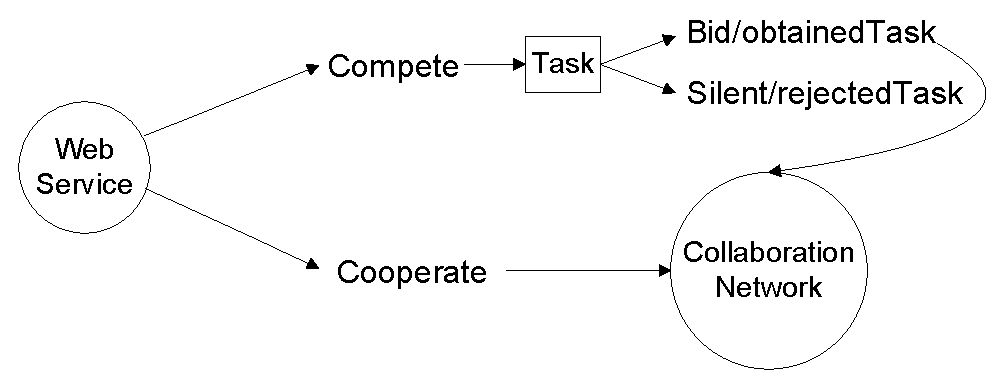
\includegraphics[scale=0.55]{Figures/decision1++.eps}
\caption{Decision making process over competitive and cooperative
strategies.} \label{decisionMakingProcedure}
\end{figure}




Consider a service $w$ that is willing to compete for the period
of time $t$ (that means the computed growth factor is more than
the analyzed threshold). This service can estimate the expected
payoff associated to this decision, called \emph{competition
payoff}. Equation \ref{CMPff} computes this expected payoff for
the competing service $w$ ($\pi_{w,CM}^t$) considering the
$Bid/obtainedTask$ probability of $p_{w,CM}^t$ and
$Silent/rejectedTask$ probability of $1-p_{w,CM}^t$.

\begin{equation}\label{CMPff}
\pi_{w,CM}^t=p_{w,CM}^t(\mu_{w, CM}E^t_w-COF_w^t
E^t_w-\epsilon)+(1-p_{w,CM}^t)(-\epsilon)
\end{equation}

In Equation \ref{CMPff}, $E^t_w$ is the number of tasks that $w$
expects during the window time $t$, and $\mu_{w, CM}$ is the mean
service fee that is assigned by the master agent to $w$. This
means that a competing service directly obtains this fee from the
master agent. Moreover, the competing service $w$ expects a
cooperation fee ($COF_w^t$) that it gives to its collaborators in
case $w$ needs to cooperate with other services (cooperative
service agents in its collaboration network). In any case, the
competing or cooperating service agent pays a fixed amount of
membership ($\epsilon$) to the master agent, which plays the role
of the community's coordinator. This fee would be taken into
account when a service decides to leave to a cheaper community or
act alone. But to concentrate on the main concerns of this thesis,
we skip these small details.\\\\
%
From Equation \ref{CMPff}, the following proposition is
straightforward.

\begin{proposition}\label{Complexity-Competition_Payoff}
The complexity of computing the competition payoff $\pi_{w,CM}^t$
is linear in the competition probability $p_{w,CM}^t$, the
expected number of tasks $E^t_w$, and the cooperation fee
$COF_w^t$.
\end{proposition}


The arrival of requests for service $w$ during the time unit $t$
(denoted here by $m_w(t)$) can be modeled as a nonhomogeneous
Poisson process \cite{DBLP:conf/icws/KhosravifarBM10,RePEc:spr:sistpr:v:8:y:2005:i:3:p:311-329}, which
means as a Poisson process with dynamic arrival rate
$\lambda_w(x)$ where $x$ belongs to the time unit $t$. The arrival
rate is thus a function of time and typically varies significantly
from moment to moment. In nonhomogeneous Poisson process, $m_w(t)$
is expressed as follows:

$$ m_w(t)= \int_0^t \! \lambda_w(x) \ \mathrm{d}x$$
%
And the probability of having exactly $n$ requests during the
window $t$ is computed as follows:

$$ p(m_w(t) = n) = \frac{(m_w(t))^n}{n! \ e^{m_w(t)}}  $$
%
Let $Max_w^t$ be the maximum number of requests that $w$ can
receive during $t$. The number of expected requests $E^t_w$ is
given by the parameter $\lambda_w(t)$ as follows:

\begin{equation}\label{Expectation}
E^t_w = \lambda_w(t) = \sum_{n=1}^{Max_w^t} n \ p(m_w(t) = n)
\end{equation}
%
The parameter $\lambda_w(t)$ is usually estimated from data
samples using the least squares, iterative least squares, or
maximum likelihood \cite{DBLP:journals/telsys/MasseyPW96}.

\begin{proposition}\label{Complexity-Expectation}
The complexity of computing the expected number of requests
$E^t_w$ is linear in the size of the window time $t$.
\end{proposition}


\begin{proof}
For a fixed function $\lambda_w(x)$, $m_w(t)$ can be computed in
$O(1)$. Thus, from Equation \ref{Expectation}, it follows that
$E^t_w$ can be computed in time linear in $Max_w^t$. As $Max_w^t$
is linear in $t$, the result follows. $\Box$
\end{proof}

Similar to the competitive service case, if a service $w$ declares
cooperative status, its expected \emph{cooperation payoff}
($\pi_{w,CO}^t$) is computed in Equation \ref{CLPff}. In this
equation, $p_{w,CO}^t$ is the probability of getting involved in a
cooperative task with other services and $1-p_{w,CO}^t$ is the
probability of failure to find such a cooperation opportunity.
These two probabilities are set when $w$ decides to compete. We
recall that $\mu_{w, CO}$ denotes the mean cooperation fee that is
directly obtained from the leader (i.e., the competitive) service
of the underlying collaborative network. Compared to $\mu_{w,
CM}$, $\mu_{w, CO}$ is relatively smaller since the competitive
service generally dedicates a portion of its obtained income to
pay other cooperative services.


\begin{equation}\label{CLPff}
\pi_{w,CO}^t=p_{w,CO}^t (\mu_{w,
CO}E^t_w-\epsilon)+(1-p_{w,CO}^t)(-\epsilon)
\end{equation}
%
From Equation \ref{CLPff}, the following proposition holds.

\begin{proposition}\label{Complexity-Cooperation_Payoff}
The complexity of computing the cooperation payoff $\pi_{w,CO}^t$
is linear in the cooperation probability $p_{w,CO}^t$ and the
expected number of tasks $E^t_w$.
\end{proposition}


To analyze the expected payoffs obtained from different
strategies, services need to compute the estimated probabilities
that distinguish subcases in each behaviorial status ($p_{w,CM}^t$
for competitive and $p_{w,CO}^t$ for cooperative). To estimate
these probabilities, we should notice that they are functions of
services' reputation values ($Rep_w^t$). Furthermore, $p_{w,CM}^t$
is also function of the difference between the offered QoS
($QoS_w^t$) and the mean requested one considering the set of all
tasks $task^t$ ($T_{QoS}^t$ (see Equation \ref{Mean-Quality}));
and $p_{w,CO}^t$ is function of the reputation of other services
in the community because the leader is supposed to be selective
when it comes to choose the collaborators. To this end, we first
discuss the desirable properties of an estimation function of each
of these probabilities, and show that the proposed ones satisfy
those properties.

\begin{equation}\label{Mean-Quality}
T_{QoS}^t =
\begin{cases} \frac{\sum_{r \in
task^t}T_{QoS}^r}{|task^t|}& \text{if $task^t \neq \emptyset$;}\\
0 & \text{otherwise.}\\
\end{cases}
\end{equation}
%

\begin{proposition}\label{Complexity-Mean_Quality}
$T_{QoS}^t$ can be computed in time linear in the size of the
window $t$.
\end{proposition}

\begin{proof}
From Equation \ref{Mean-Quality},  $T_{QoS}^t$ can be computed in
time linear in $|task^t|$, which in turn is linear in the window
size $|t|$. $\Box$

\end{proof}


The desired properties of $p_{w,CM}^t$ are as follows:

\begin{property}
$p_{w,CM}^t$ is continuous with regard to $Rep^t_w$, $QoS_w^t$,
and $T_{QoS}^t$.
\end{property}
%
\begin{property}
$p_{w,CM}^t$  is monotonically increasing in $Rep^t_w$ and
$QoS_w^t - T_{QoS}^t$ while $QoS_w^t - T_{QoS}^t$ is positive.
\end{property}
%
\begin{property}
$p_{w,CM}^t$ is null if $QoS_w^t - T_{QoS}^t$ is negative.
\end{property}
%
%\begin{property}
%Assuming that the web service $w$ is known by the master web
%service, $Rep^t_w$ is monotonically increasing or decreasing in
%$QoS_w$.
%\end{property}
%
\begin{property}
The increase slope of $p_{w,CM}^t$ is higher when the reputation
$Rep^t_w$ increases in the interval $[0, 0.5]$ than when it
increases in the interval $]0.5, 1]$.
\end{property}


\noindent Property 1 simply says that the probability of success
competition $p_{w,CM}^t$ can be always estimated as far as
$Rep^t_w$, $QoS_w^t$, and $T_{QoS}^t$ are available. Property 2
says that the reputation and QoS are two key factors that
influence the value of $p_{w,CM}^t$ in the sense of positive
correlation. Property 3 indicates that the probability
$p_{w,CM}^t$ is null if the offered QoS is less than the
expectation. Property 4 promotes the increase of the reputation
for new comers and imposes higher increase rate at the beginning
of the reputation curve because it is always hard to build the
reputation, but once it is built, its maintenance is less
challenging.


\noindent The desired properties of $p_{w,CO}^t$ are as follows:

\begin{property}
$p_{w,CO}^t$ is continuous with regard to $Rep^t_w$ and the
reputation of other services in the community.
\end{property}
%
\begin{property}
$p_{w,CO}^t$  is monotonically increasing in $Rep^t_w$ and
 monotonically decreasing in the community average reputation.
\end{property}
%
%\begin{property}
%$p_{w,CM}$ is null if $QoS_w^t - T_{QoS}^t$ is negative.
%\end{property}
%
%\begin{property}
%Assuming that the web service $w$ is known by the master web
%service, $Rep^t_w$ is monotonically increasing or decreasing in
%$QoS_w$.
%\end{property}
%
\begin{property}
The increase slope of $p_{w,CO}^t$ is higher when the reputation
$Rep^t_w$ increases in the interval $[0, 0.5]$ than when it
increases in the interval $]0.5, 1]$.
\end{property}

\noindent Property 5 is similar to Property 1. Property 6 says
that $w$ has more chance to get involved in a cooperation if it
has high reputation compared to the other members. This chance
decreases if other services have higher reputation. Property 7 is
similar to Property 4.

Equations  \ref{CMp_w} and \ref{CLp_w} respectively compute the
estimated success probability in cases where service $w$ is
competing and cooperating. These values are computed considering
service's reputation value ($Rep^t_w$ computed by the master),
service's offered QoS ($QoS^t_w$), the task required QoS
($T_{QoS}^t$), which is the mean required QoS computed from
previous tasks, the maximum offered QoS ($QoS_k^t$, which is
provided by another competitive service $k$), and the cooperative
factor $CL_w^t$ of service $w$ during the window time $t$, which
is computed as the portion of service's current reputation on the
average reputation of the community $\mathcal{C}$.

\begin{equation} \label{CMp_w}
p_{w,CM}^t = \begin{cases}
\sin(Rep^t_w\frac{\pi}{2})\frac{QoS_w^t-T_{QoS}^t}{Max_k(Qos_k^t-T_{QoS}^t)} & \text{if $QoS_w^t\geq T_{QoS}^t$;}\\
0 & \text{otherwise.}\\
\end{cases}
\end{equation}

\begin{equation}\label{CLp_w}
p_{w,CO}^t=\sin(Rep^t_w\frac{\pi}{2})CL_w^t
\end{equation}
\begin{equation*}
CL_w^t=\frac{Rep^t_w}{\sum_{k\in
\mathcal{C}}Rep^t_k/|\mathcal{C}|}
\end{equation*}

\begin{theorem}
Equation  \ref{CMp_w} satisfies Properties 1 to 4.
\end{theorem}

\begin{proof}
It is easy to show the continuity of Equation \ref{CMp_w}, which
satisfies Property 1. The partial derivative $\frac{\partial
p_{w,CM}^t}{\partial Rep^t_w} = \frac{\pi}{2}
\cos(Rep^t_w\frac{\pi}{2})\frac{QoS_w^t-T_{QoS}^t}{Max_k(Qos_k^t-T_{QoS}^t)}$
is positive as the function $\cos$ (the derivative of $\sin$) is
positive on $[0, \frac{\pi}{2}]$, $Rep^t_w \in [0, 1]$, and
$QoS_w^t\geq T_{QoS}^t$. The partial derivative $\partial
p_{w,CM}^t$ with regard to $QoS_w^t - T_{QoS}^t$ ($\frac{\partial
p_{w,CM}^t}{\partial(QoS_w^t - T_{QoS}^t)} =
\frac{\sin(Rep^t_w\frac{\pi}{2})}{Max_k(Qos_k^t-T_{QoS}^t)}$) is
also positive since $Qos_k^t-T_{QoS}^t > 0$ and
$Rep^t_w\frac{\pi}{2} \in [0, \frac{\pi}{2}]$ and $\sin$ is
positive on $[0, \frac{\pi}{2}]$, which proves the satisfaction of
Property 2. Property 3 is straightforward. Finally, the increase
slope of the function $\sin$ on $[0, \frac{\pi}{2}]$ proves
Property 4. $\Box$
\end{proof}

\begin{theorem}
Equation  \ref{CLp_w} satisfies Properties 5 to 7.
\end{theorem}
%
\begin{proof}
We can easily show the continuity  of Equation \ref{CLp_w} from
which Property 5 follows. Property 6 can be shown by calculating
the partial derivative $\partial p_{w,CO}^t$ first with regard to
$Rep^t_w$ and second with regard to the community $\mathcal{C}$
average reputation $\sum_{k\in \mathcal{C}}Rep^t_k/|\mathcal{C}|$,
where $|\mathcal{C}|$ is the cardinality of the considered
community $\mathcal{C}$. The first partial derivative
($\frac{\pi}{2}\cos(Rep^t_w\frac{\pi}{2})CL_w^t$) is positive and
the second ($\frac{-\sin(Rep^t_w\frac{\pi}{2})Rep^t_w}{(\sum_{k\in
\mathcal{C}}Rep^t_k/|\mathcal{C}|)^2}$) is negative, which proves
the satisfaction of Property 6. The proof of satisfaction of
Property 7 is similar to the one of Property 4. $\Box$
\end{proof}
%Considering these involved parameters, we verify that properties
%$1$ to $3$ are satisfied. For property $4$, we use $sinus$
%function to promote the role of reputation influence in this
%system. Using $sinus$ function, we promote reputation increase of
%web services specially when it is less than $50\%$. Considering
%the desired properties, the formulas represented in Equations
%\ref{CMp_w} and \ref{CLp_w} are candidates we chose to compute the
%probabilities regarding $Competitive$ and $Cooperative$
%strategies. These formulas are used in implemented system and
%verified with respect to their accuracy and effectiveness in
%adopting different interacting strategies.


%In the proposed heuristic  function, the web service $w$ is not
%aware of current $T_{QoS}$ and $QoS_k$, but could use its previous
%information to estimate their values. To this end, if the web
%service is more informative about the previous data, it could
%obtain more realistic measurement over the estimated
%probabilities.
%
%
%We compute the success probability of cooperation ($p_{w,CO}$)
%similarly in the sense  that we still promote reputation influence
%using $sinus$ function, but multiplied to the cooperative factor
%$CL_w$ of the web service $w$. This value is computed as the
%portion of web service's current reputation on the average
%reputation of the community.



\begin{proposition}\label{Complexity-Probability_Competition}
$p_{w,CM}^t$ can be computed in time linear in the window size
$|t|$.
\end{proposition}

\begin{proof}
The result follows directly from 1) Equation \ref{CMp_w}; 2)
Proposition \ref{Complexity-Rep} (Complexity of $Rep^t_w$ is
linear in the window size $|t|$); 3) second part of Equation
\ref{eq:growthfactor} (the function $QoS_w^t$ can be computed in
time linear in the number of tasks, which in turn is linear in the
size of the window time); 4) Proposition
\ref{Complexity-Mean_Quality} (Complexity of $T_{QoS}^t$ is linear
in the size of the window $t$); and 5) the fact that those
functions are computed independently one from the other. $\Box$
\end{proof}



\begin{proposition}\label{Complexity-Probability_Cooperation}
$p_{w,CO}^t$ can be computed in time $O(|t|.|\mathcal{C}|)$, which
means linear in both the size of the window $t$ and the size of
the community $\mathcal{C}$.
\end{proposition}

\begin{proof}
From Proposition \ref{Complexity-Rep}, $Rep^t_w$ can be computed
in $O(|t|)$. Consequently, the function $\sum_{k\in
\mathcal{C}}Rep^t_k$ can be computed in $O(|t|.|\mathcal{C}|)$, so
it does the computation of the function $CL_w^t$ as $Rep^t_w$ will
be computed just once and stored in a variable. The same variable
will be used to compute $\sin(Rep^t_w\frac{\pi}{2})$. Thus, from
Equation \ref{CLp_w}, the result follows. $\Box$
\end{proof}


\subsection{Coopetition Threshold}

In this part, we compute the coopetition threshold that a typical
service agent could use to adopt reasonable interacting strategies
and we empirically verify the effectiveness of the obtained
results in the next section. In fact, to decide which strategy to
adopt, we let the service agent $w$ compare its growth factor
$G_w^t$ with the coopetition threshold $\tau_w^t$ it holds at
current window time $t$ and choose to compete with probability
$P_w^t$ that we compute in Equation \ref{P}. Based on this
probability, we calculate the total utility $U_w^t$ in Equation
\ref{U}.

\begin{equation} \label{P}
P_w^t= \begin{cases}
\frac{G_w^t}{\tau_w^t}  & \text{if $G_w^t\leq \tau_w^t$;}\\
1 & \text{otherwise.}\\
\end{cases}
\end{equation}

\begin{equation}\label{U}
U_w^t=P_w^t(\pi_{w,CM}^t)+(1-P_w^t)(\pi_{w,CO}^t)
\end{equation}


%Equation  \ref{U} computes the
%expected utility (as accumulated fee) regarding web service $w$.
%This estimated utility is result of aggregation of two different
%interacting strategies of $Competitive$ and $Cooperative$.
%Aggregating these strategic payoffs, web service $w$ follows
%probability distribution of $\{P,1-P\}$. This probability
%distribution is computed in Equation \ref{P}, which is a function
%of the growth factor ($G_w$) and computed threshold ($Tr^t$). So
%if the web service is aware of the reasonable threshold, the value
%$p$ could be computed and used as the core of strategic
%probability distribution. But there is a case where the web
%service does not have a reasonable threshold value and cannot
%rigorously decide for any adopting strategies.


The key factor in the computation of the probability $P_w^t$ and
the associated utility is the threshold value. To compute the
threshold, we use the game-theoretic best response technique. A
typical service agent $w$ will follow the best response strategy
to maximize its expected aggregated payoff. The idea is to
equalize the expected payoffs of the two acting strategies:
compete and cooperate.
%
%
%by following the following three probability distributions: (1)
%$\{1,0\}$ where the web service always competes; (2) $\{0,1\}$
%where the web service always cooperates; and (3)
%$\{\frac{1}{2},\frac{1}{2}\}$ where the web service equalize the
%probabilities and decides with unbiased distribution. Following
%the third case, the web service equites the expected payoffs as
%outcomes of different interacting strategies.
%
The objective behind equalizing payoffs is to explore conditions
under which service agent $w$ could react with best response to
further decision making procedures. We use the obtained conditions
to compute the threshold $\tau_w^t$ during the window time $t$. By
equalizing $\pi_{w,CM}^t$ and $\pi_{w,CO}^t$, we obtain:

\begin{equation*}\label{equit}
\pi_{w,CM}^t=\pi_{w,CO}^t      \rightarrow
\end{equation*}
\begin{equation*}
p_{w,CM}^t(\mu_{w,CM}-COF_w^t-\epsilon)+(1-p_{w,CM}^t)(-\epsilon)=p_{w,CO}^t(\mu_{w,
CO}-\epsilon)+(1-p_{w,CO}^t)(-\epsilon)
\end{equation*}
Which means:
\begin{equation*}
p_{w,CM}^t(\mu_{w,CM}-COF_w^t - \epsilon) =
p_{w,CO}^t(\mu_{w,CO}-\epsilon)+(-\epsilon)(p_{w,CM}^t -
p_{w,CO}^t)
\end{equation*}
So, we obtain:
\begin{equation*}
\mu_{w,CM}-COF_w^t - \epsilon =
\frac{p_{w,CO}^t~~\mu_{w,CO}}{p_{w,CM}^t}-\epsilon
\end{equation*}
Therefore:
\begin{equation*}
\mu_{w,CM}-COF_w^t = \frac{p_{w,CO}^t~~\mu_{w,CO}}{p_{w,CM}^t}
\end{equation*}
From which, we derive:
\begin{equation*}
COF_w^t = \mu_{w,CM} - \frac{p_{w,CO}^t~~\mu_{w,CO}}{p_{w,CM}^t}
\end{equation*}
Replacing $p_{w,CM}^t$ and $p_{w,CO}^t$ using Equations
\ref{CMp_w} and \ref{CLp_w}, we derive the following:
\begin{equation*}
COF_w^t = \mu_{w,CM} -
\frac{sin(Rep^t_w\frac{\pi}{2})CL_w^t~~\mu_{w,CO}}{sin(Rep^t_w\frac{\pi}{2})\frac{QoS_w^t-T_{QoS}^t}{Max_k(Qos_k-T_{QoS}^t)}}
\end{equation*}
%The fixed membership fee $\epsilon$ could be taken out and
%canceled from both sides of the equation so we obtain the
%following:
%\begin{equation*}
%p_{w,CM}^t(\mu_{w,CM}-COF_w^t)=p_{w,CO}^t(\mu_{w,CO})\rightarrow
%\end{equation*}
%
%\begin{equation*}
%sin(Rep^t_w\frac{\pi}{2})\frac{QoS_w^t-T_{QoS}^t}{Max_k(Qos_k-T_{QoS}^t)}(\mu_{w,
%CM}-COF_w^t)=sin(Rep^t_w\frac{\pi}{2})CL_w^t(\mu_{w, CO})
%\end{equation*}
By simplifying the $sinus$ function from both the numerator and
denominator sides and substituting the cooperation factor $CL_w^t$
of service $w$ we obtain Equation \ref{CLF}:

\begin{equation}\label{CLF}
COF_w^t=\mu_{w,CM}-\frac{Rep^t_w~|\mathcal{C}|}{\sum_{k\in
\mathcal{C}}Rep^t_k}\frac{\mu_{w,CO}Max_k(Qos_k^t-T_{QoS}^t)}{QoS_w^t-T_{QoS}^t}
\end{equation}

Equation \ref{CLF} computes the cooperation fee $COF_w^t$ that is
assigned by service $w$. This fee represents the amount that $w$
spends to cooperate with other service(s) to accomplish the task.
By so doing, we obtain the maximum amount of cooperation fee that
service $w$ can use to constrain the positive payoff out of
competing. Otherwise, the service stays as cooperative entity.

\begin{proposition}\label{Complexity-COF}
$COF_w^t$ can be computed in time $O(|t|.|\mathcal{C}|)$, which
means linear in both the size of the window $t$ and the size of
the community $\mathcal{C}$.
\end{proposition}

\begin{proof}
From Proposition \ref{Complexity-Rep}, $Rep^t_w$ can be computed
in $O(|t|)$. Consequently, the function $\sum_{k\in
\mathcal{C}}Rep^t_k$ can be computed in $O(|t|.|\mathcal{C}|)$.
Since $QoS_w^t$ and $T_{QoS}^t$ can be computed in time $O(t)$
(from the second part of Equation \ref{eq:growthfactor} and
Proposition \ref{Complexity-Mean_Quality} respectively), we are
done. $\Box$
\end{proof}

\begin{lemma} \label{Complexity-Competition_Payoff-Final}
The competition payoff $\pi_{w,CM}^t$ can be computed in time
$O(|t|.|\mathcal{C}|)$.
\end{lemma}

\begin{proof}
The result follows directly from Propositions
\ref{Complexity-Competition_Payoff}, \ref{Complexity-Expectation},
\ref{Complexity-Probability_Competition}, and
\ref{Complexity-COF}. $\Box$
\end{proof}

\begin{lemma} \label{Complexity-Cooperation_Payoff-Final}
The cooperation payoff $\pi_{w,CO}^t$ can be computed in time
$O(|t|.|\mathcal{C}|)$.
\end{lemma}


\begin{proof}
The result follows directly from Propositions
\ref{Complexity-Expectation}, \ref{Complexity-Cooperation_Payoff},
and \ref{Complexity-Probability_Cooperation}. $\Box$
\end{proof}




%\begin{equation*}
%\frac{QoS_w^t-T_{QoS}^t}{Max_k(Qos_k^t-T_{QoS}^t)}(\mu_{w,CM}-COF_w^t)=\frac{Rep^t_w}{\sum_{k\in
%Community}Rep^t_k}(\mu_{w, CO})
%\end{equation*}
%



We use the maximum cooperation fee that a service agent considers
to constrain the positive expected payoff when the competitive
strategy is adopted to update the threshold for the consequent
time window ($t+1$). We compare the maximum cooperation fee with
the required fee ($ReqF_w^t$) that the service indicates to
accomplish the task. The outcome of this comparison is a factor
that uses the current threshold $\tau_w^t$ to compute the
consequent threshold $\tau_w^{t+1}$. As in online learning, the
idea is to compute iteratively the threshold until the fixed point
is achieved, which indicates the threshold's conversion, where the
initial value is randomly chosen (in the simulation different
initial values are used). Equation
\ref{Trt} shows this computation. %We restrict the range of this value to $(0.15,0.85)$ to
%avoid some unreasonable results that could occur due to different
%reasons like system start point or heavy loaded competitive web
%services, \textit{etc}.
To investigate the effectiveness of this threshold on the outcomes
of the services that follow this reasoning technique, in the next
section, we compare the results of different agents with diverse
strategic reasoning techniques.

\begin{equation}\label{Trt}
\tau_w^{t+1}=\begin{cases}
\Theta & \text{if $0 \leq \Theta \leq 1$}\\
1 & \text{if $\Theta > 1$;}\\
0 & \text{if $\Theta < 0$.}\\
\end{cases}
\end{equation}
\begin{equation*}
\Theta =\tau_w^t \ \frac{COF_w^t}{ReqF_w^t}
\end{equation*}


\begin{proposition}\label{Complexity-Threshold}
The threshold $\tau_w^{t}$ can be computed in time
$O(|t|.|\mathcal{C}|)$, which means linear in both the size of the
window $t$ and the size of the community $\mathcal{C}$.
\end{proposition}

\begin{proof}
From Equation \ref{Trt}, the computation of $\tau_w^{t}$ is
recursive on $t$, and the algorithm works by keeping the last
computed value in a variable, which saves the time of
re-calculation. Thus, the complexity of calculating $\tau_w^{t}$
is determined by the complexity of calculating $COF_w^t$ since
$ReqF_w^t$ is constant during the period $t$. Consequently, the
result follows from Proposition \ref{Complexity-COF}. $\Box$
\end{proof}


\begin{theorem}\label{Complexity-Procedure}
The time complexity of the proposed decision mechanism is
$O(|t|.|\mathcal{C}|)$, which means linear in both the size of the
window $t$ and the size of the community $\mathcal{C}$.
\end{theorem}

\begin{proof}
The procedure mechanism is based on comparing the growth factor
$G_w^t$ with the coopetition threshold $\tau_w^t$ as shown in
Equations \ref{P} and \ref{U}. Thus, the result follows from
Propositions \ref{Complexity-Growth_Factor} and
\ref{Complexity-Threshold}. $\Box$
\end{proof}



\section{Experimental Results and Analysis}\label{s4:resutls}

In this section, we provide an empirical analysis over the
theoretical results regarding the characteristics of intelligent
service agents hosted in different communities of services. In the
implemented system, we simulate the behaviors of service consumers
as request generators, service agents as service providers, and
master agents as community representatives.
%These entities are developed with respect to what is explained in Section \ref{s4:Preliminaries}.
The objective is to investigate the effectiveness of the proposed strategic system on
intelligent services' overall budget and also the average quality
and quantity of tasks performed by the community of services,
which directly affects user satisfaction.
%Before conducting the simulation, the
%expected behavior of our model is to enhance the budget of web
%services when using our proposed strategic interacting system.
%Although this result is promising, we would like to investigate
%the effectiveness of the proposed strategic system on intelligent
%web services' overall budget compared to the best case. Moreover,
To verify these objectives, we study the overall performance of
the community hosting the reasoning-empowered services compared to
the ones hosting stochastic and purely competitive services. By
stochastic services, we mean services that adopt at each moment
competitive or cooperative strategies in an equally but random
way. By equally, we mean the choices are fairly divided between
the two strategies.

The simulation application is written in
\textit{C\#} using \textit{Visual Studio}. We performed the implementation on a single Intel Xeon X3450 machine with 6GBs of memory. Web services were modeled as a \emph{class} and using \emph{Await} and \emph{Async} models we initiated many web services, each running as a thread.  We implemented XML based messaging system (like SOAP) with request parameters and a list of XML based responses. The request contains the flight dates, the origin and destination, type of tickets, and number of guests. The response contains different flights with different companies, prices, timing, etc. A pool of services are initialized with values taken from a real dataset that includes $2507$ real services functioning on the web.
The dataset records the QoS values of $9$ parameters including \textit{availability},
\textit{throughput}, and \textit{reliability} \cite{DBLP:conf/www/Al-MasriM07a}.

We start our discussions with cumulative budget comparison
regarding different communities within which services follow
different reasoning techniques. Figure \ref{Graph1} part (a)
illustrates three graphs for three different communities. Each
community hosts services that follow different reasoning
techniques: (1) a community that follows the interactive reasoning
techniques presented in this report (referred to as coopetitive);
(2) a community that follows a stochastic reasoning technique so
decisions about selecting competitive or cooperative strategies
are totally random (referred to as random coopetitive); and (3) a
competitive community where all services follow the competitive
strategy (referred to as competitive).
%The proposed model's
%reasoning mechanism allows services to make decisions that
%maximize their utilities, so that if the service cannot compete,
%the procedure would suggest to collaborate, which is better than
%competing and failing to obtain the task. In this case, the service stays idle but
%still pays the community membership fee, which means losing
%utility. The developed strategic decision making mechanism leads
%some service agents to follow cooperative strategies that overall
%maintain an optimal community budget. In the same figure, we
%observe the cumulative budget of a community where services follow
%random interacting strategies. The outcome is clearly lower
%because services at each run randomly decide over their acting
%strategies. This potentially influences the community budget
%because a low quality service if randomly selects to follow the
%competitive strategy, it will fail to perform a task with high QoS
%requirements.


The results illustrated in Figure \ref{Graph1} part (a)  verify
the importance of the strategic decision making procedure to
logically decide over the possible competitive and cooperative
choices. Figure \ref{Graph1} part (b) illustrates communities
average reputation of involved services. The graphs represent the
influence of the rewards that the master agent uses to encourage
highly capable services to compete for a task. As for the
cumulative budget, we observe that the coopetitive community
outperforms the random coopetitive and competitive communities in
terms of average reputation. The proposed model's average
reputation increases because services follow optimal strategies
where they can perform better so obtain higher rewards. For the
same reasons as for the cumulative budget, the average reputation
of the random coopetitive community
outperforms the one of the competitive community. %The idea is to balance web
%services' strategies to maintain optimal community budget.


\begin{figure}%[h]
%\centering
%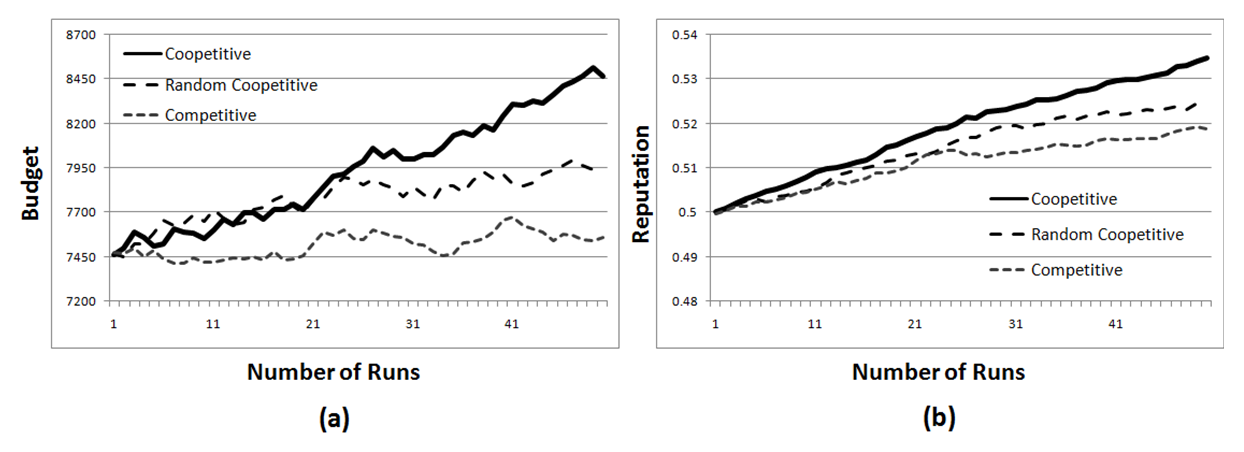
\includegraphics[scale=0.6]{graph1Final+.eps}
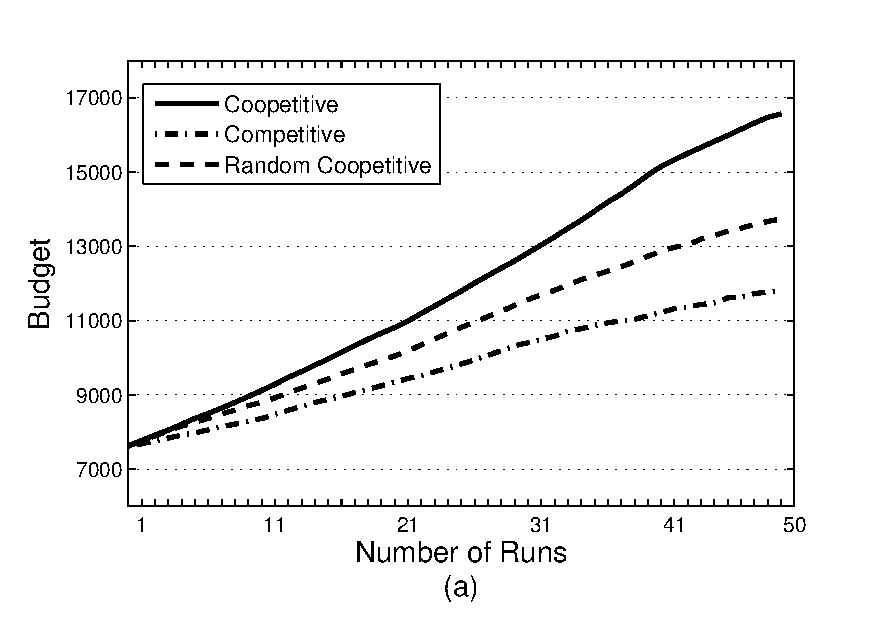
\includegraphics[scale=0.55]{Figures/graphbgtmed.eps}
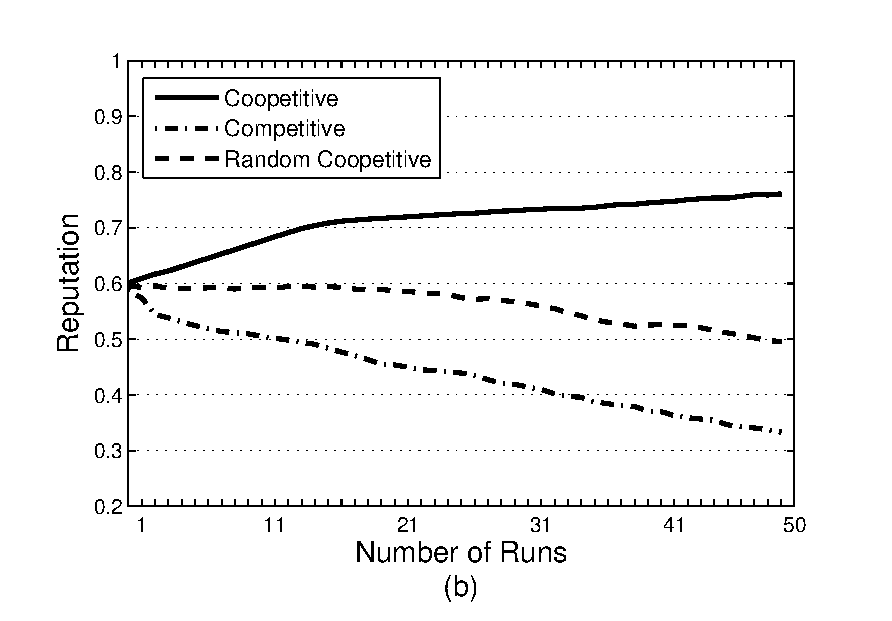
\includegraphics[scale=0.55]{Figures/graphrep.eps}
\caption{Part (a): Cumulative community budget comparison. Part
(b): Average community reputation comparison over different
strategic decisions.} \label{Graph1}
\end{figure}



 %Figure \ref{Graph2} part (a) illustrates the reputation of the proposed $Coopetitive$ community where
 %we highlight the range of reputation change in the community. The vertical lines denote the range of %reputation that is associated with the master web service. The rewards and penalties applied to %different
% web services show that the master web service over runs extends the reputation range and takes %control of the whole community. In the developed model, web services are encouraged to choose
 %optimal strategies. This is maintained over growth factor comparison of the $Coopetitive$ web %services.


In our model, services are managed by selfish agents in the sense
they try to maximize their own utilities. We analyze how their
strategies affect the social welfare, and from user's and
community's point of view how good the tasks are being performed.
This directly impacts user's satisfaction and community's
reputation in general. The Higher quality and quantity of tasks
performed leads to higher user's satisfaction for the community
which results in better reputation for the community. The results
in Figure \ref{graph_task} show the quality and quantity of tasks
being done successfully in three communities adopting the three
different aforementioned strategy decision algorithms. As clearly confirmed by the simulation, the coopetitive community
outperforms the stochastic and compete communities.

\begin{figure}[h]
\centering
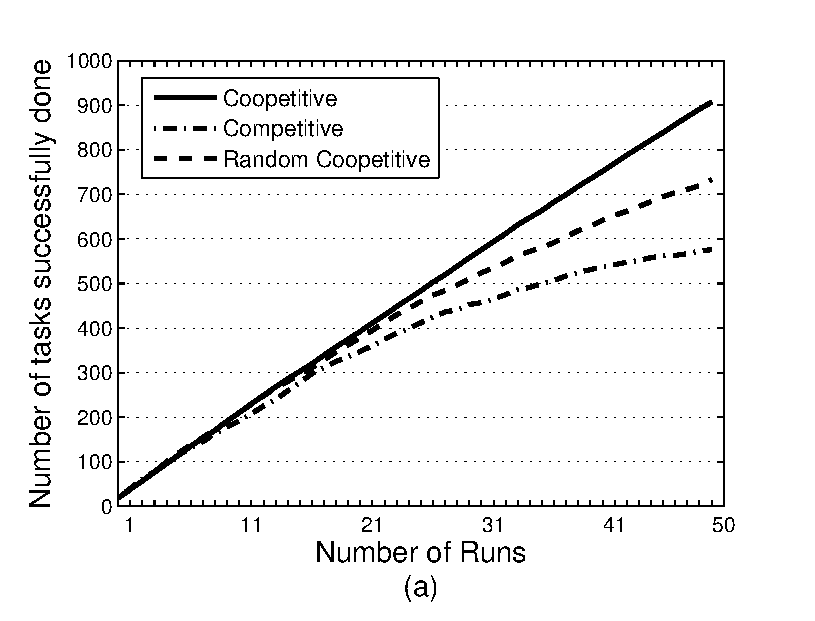
\includegraphics[scale=0.55]{Figures/graphtaskdone.eps}
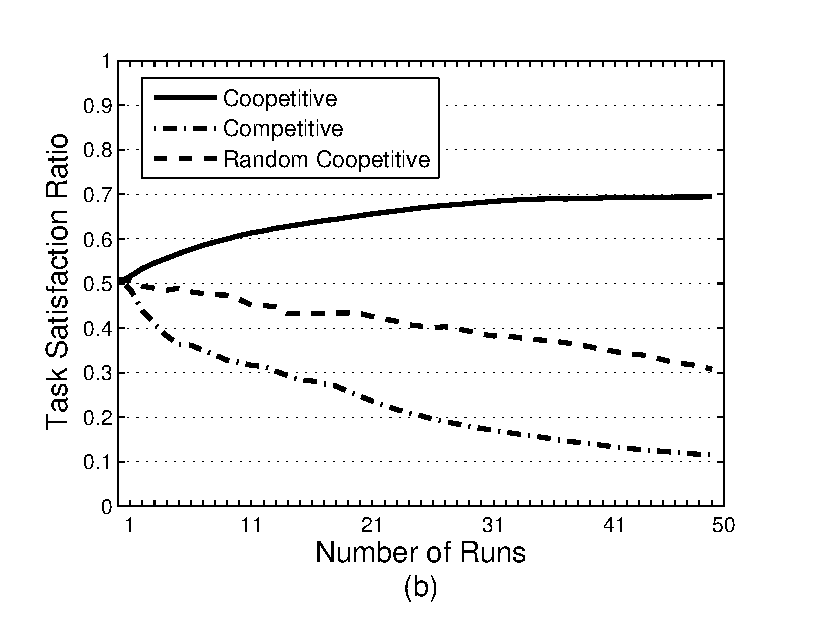
\includegraphics[scale=0.55]{Figures/graphtasksatisfaction.eps}
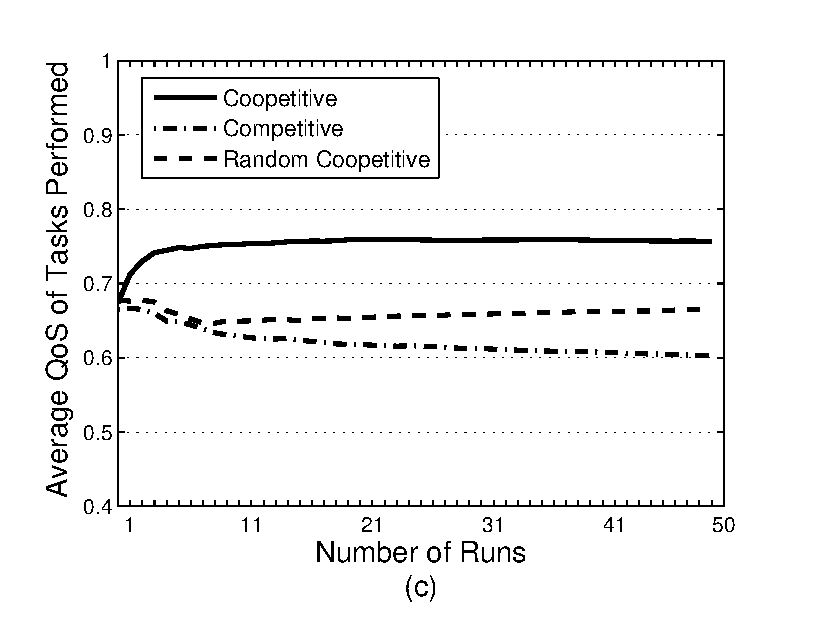
\includegraphics[scale=0.55]{Figures/graphavgqostask.eps}
\caption{Overall performance from community's point of view. Part
(a) Total number of tasks successfully done. Part (b) Ratio of
tasks satisfied with required QoS. Part (c) Average QoS of
performed tasks.} \label{graph_task}
\end{figure}


We conclude our analysis by discussing how effective our
coopetitive decision making model is by comparing the final
utility (in terms of income) of services following our model with
other services deviating from that coopetitive model. In Figure
\ref{graph_dev} Part (a), we made the services deviate from the
suggested strategy. As the simulation shows, the more services
deviate from our coopetitive strategy the more they make less
benefits. In Part (b), we pick one random service and simulate the
scenario with its default coopetitive strategy and then we redo
the simulation with exactly the same environment parameters while
gradually alternating the decisions. By alternating we mean
adapting the opposite of what our model does suggest. Thus, if the
coopetitive model suggests to compete, the service agent will
cooperate and vice versa. We run this scenario 50 times and at the
end we check the service's budget and see if it gains more by
deviating or not. We did this for one single deviation (i.e.,
alternating only one decision) to 10 different deviations
(alternating 10 different decisions) during the 50 times run. As
the results show, deviating from the coopetitive strategy yields
less income for the service.

\begin{figure}%[h]
%\centering
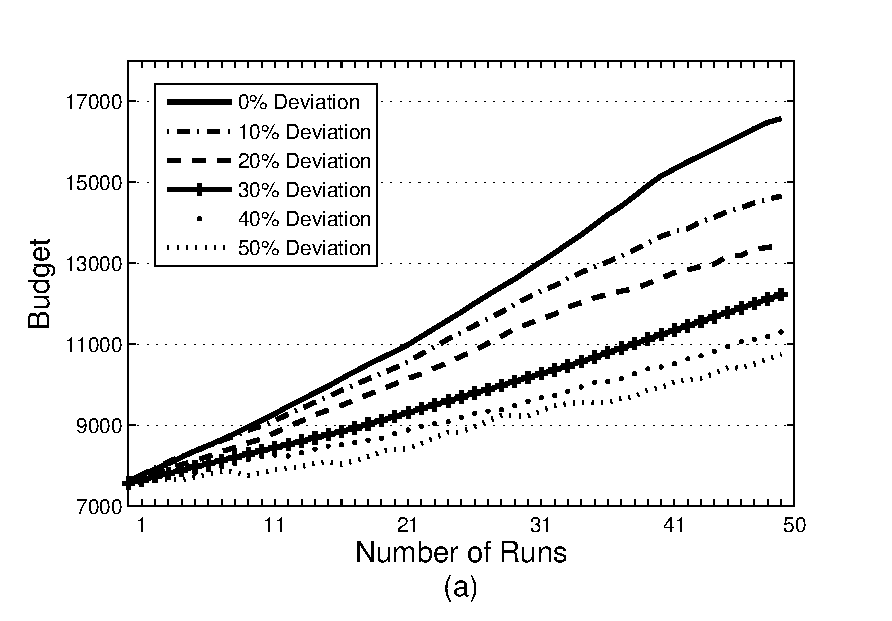
\includegraphics[scale=0.55]{Figures/graphdev.eps}
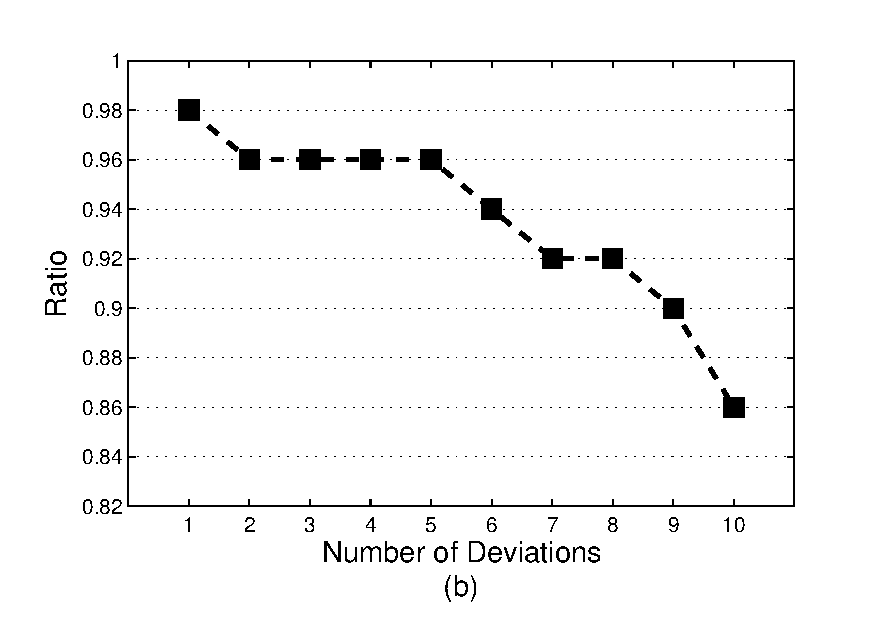
\includegraphics[scale=0.55]{Figures/graphdev2.eps}
\caption{Utility loss while deviating from our coopetitive
decision process. Part (a) Overall budget when deviating from our
model in 0, 10, 20, 30, 40, and 50 percent of decisions. Part (b)
Ratio of getting earning utility (budget) when deviating from our
coopetitive strategy in 1 to 10 decisions.} \label{graph_dev}
\end{figure}

%%%%%%%%%%%%%%%%%%%%%%%%%%%%%%%%%%%%%%
\section{Summary}\label{sec:conclusion-cha3}

In this chapter, we proposed a game-theoretic based model to analyze the efficiency characteristics for the active services in open networks. The proposed framework considers the chances of web services in joining a community in different cases with truthful and lying information service agents. The proposed game analyzes the existing Nash equilibrium and situations where the maximum payoff is obtained.

Our model has the advantage of being simple and taking into account three important factors: (1) rational web services seek better status in the environment by joining the community; (2) rational web services obtain higher payoff by truth telling; and (3) the community is obtaining more effective web services. These advantages are confirmed through the conducted simulations.
%As future work, we plan to consider the user role in the game to obtain more accurate results when users act rationally. Moreover, we would like to achieve a collusion resistant efficiency mechanism, which is still an open problem in open environments.
